
\def\Ponderation{40}
\def\SigleNumero{STT-1900}
\def\NomCours{Méthodes statistiques pour ingénieurs}
\def\DateEvaluation{20 octobre 2023}
\def\HeureEvaluation{18h30 à 21h30}
\def\Session{}
\def\NomEvaluation{Examen 1}

% Ne rien mettre entre les accolades si l'enseignant (ou l'enseignante) est aussi le coordonnateur (ou la coordonnatrice)
\def\Coordonnatrice{}
\def\Coordonnateur{}

% Ne rien mettre entre les accolades s'il y a plus d'une section
\def\Enseignant{}
\def\Enseignante{}

% Ne rien mettre entre les accolades s'il s'agit d'un cours à section unique
% Mettre le nom de chacun des enseignants et enseignantes entre les accolades
% Une case à cocher sera générée pour chacune des sections
\def\SectionA{Ahmed Sid-Ali}
\def\SectionB{Julien Miron}
\def\SectionC{}
\def\SectionD{}


\def\Directives{
\begin{enumerate}
\item Matériel autorisé:
\begin{itemize}
    \item Calculatrice scientifique {\bf autorisée par la faculté des sciences et de génie};
    \item Une seule feuille aide-mémoire \textbf{manuscrite} de format lettre (8.5''$\times$11'') recto-verso.
    \end{itemize}
\item Assurez-vous que cette évaluation comporte \numquestions ~questions réparties sur \numpages{}~pages, pour un total de \numpoints{}~points.\
\item \textbf{Veuillez ne pas dégrafer votre examen.}
\item Les tables de lois se trouvent dans un deuxième feuillet. SVP, ne rien écrire sur les tables.
\item Ajoutez vos initiales dans le bas de chaque page.
\item Veuillez déposer votre carte d'identité \textbf{admise} avec photo sur votre bureau.\
\item Vous devez\textbf{ justifier toutes vos réponses} par une démarche claire, sauf pour les questions à choix de réponse et les vrais ou faux.\
\item Pour les questions à choix de réponse et les vrais ou faux, vous pouvez mettre un X, un crochet ($\checkmark$) ou remplir la case.
\item Le verso des feuilles peut être utilisé comme brouillon, \textbf{mais ne sera pas corrigé}. Attention à ne rien dégrafer.
\end{enumerate}
}



\documentclass{Evaluation}
\usepackage{multicol,graphicx}
\begin{document}

\newpage . \newpage
%%%%%%%%%%%%%%%% QUESTION %%%%%%%%%%%%%%%%
\begin{questions}

\question[3] Laquelle des fonctions suivantes est une fonction de densité? 

\begin{checkboxes}
\choice $f(a)=a,\ \mbox{pour } 0 <a$
		\vspace{0.3cm}
\correctchoice $ f(b) = \left\{
			\begin{array}{ll}
			0  & \mbox{ si } b<0, \\
			b & \mbox{ si } 0\leq b < 2,\\
			0 & \mbox{ si } 2 \leq b
			\end{array}
			\right. $
\choice $ f(c) = \left\{
			\begin{array}{ll}
			\sqrt{c}  & \mbox{ si } 0\leq c\leq 1, \\
			0 & \mbox{sinon}
			\end{array}
			\right. $
\choice $ f(d) = \left\{
			\begin{array}{ll}
			0  & \mbox{ si } d < 0, \\
			d & \mbox{ si } 0 \leq d \leq 1,\\
			1 &  \mbox{ si } 1 < d
			\end{array}
			\right. $
\end{checkboxes}



\question[3] Laquelle des affirmations suivantes est toujours vraie au sujet de $\overline{X}=\displaystyle \frac{1}{n}\sum_{i=1}^n X_i$, où les $X_i$ sont indépendants et identiquement distribués de loi quelconque d'espérance $\mu_X$ et de variance $\sigma^2_X$? %module 5

\begin{checkboxes}
\choice $\displaystyle Z=\frac{\overline{X}-\mu_X}{\sigma_X / \sqrt{n}}\sim \mathcal{N}(0, 1)$

\choice $\mathbb{E}\left[\overline{X}\right]=\mu_X$ seulement si $n>30$
\vspace{0.1cm}
\correctchoice $\mathbb{E}\left[\overline{X}\right]=\mu_X$ peu importe la loi des $X_i$
\vspace{0.1cm}
\choice $\displaystyle\mathbb{E}\left[\overline{X}\right]=\mu_X$  seulement si les $X_i$ sont de loi normale
\vspace{0.1cm}
\choice $\text{Var}\left[\overline{X}\right]=\sigma^2_X$
\end{checkboxes}

\vspace{0,5cm}


\question[3]\label{probaQCM} Considérons le montage électronique représenté ci-dessous.
	
\begin{figure}[h!]
    \label{fig:montage}
    \begin{center}	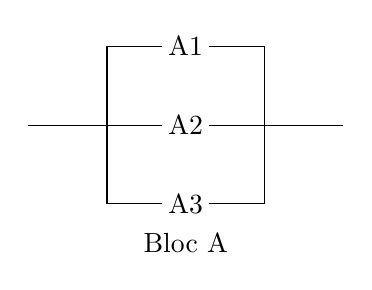
\begin{tikzpicture}	
		% bandes extérieures
		\draw (0,0)--(1,0);
            \draw (3,0)--(4,0);

            % étiquette éléments
		\node at (2,1) {A1};
		\node at (2,0) {A2};
            \node at (2,-1) {A3};
            
            % vers les étiquettes
            \draw (1,1) -- (1.7,1); %vers A1
            \draw (1,0) -- (1.7,0); %vers A2
            \draw (1,-1) -- (1.7,-1); %vers A3
            
            % à partir des étiquettes
            \draw (2.3,1) -- (3,1); %de A1
            \draw (2.3,0) -- (3,0); %de A2
            \draw (2.3,-1) -- (3,-1); %de A3

            %premiers verticaux
            \draw (1,0) -- (1,1); % A1
            \draw (1,0) -- (1,-1); % A3

            %deuxièmes verticaux
            \draw (3,0) -- (3,1); % A1
            \draw (3,0) -- (3,-1); % A3
		
		\node at (2,-1.5) {Bloc A};
    \end{tikzpicture} \end{center}
\end{figure}
	
 Le bloc A contient trois éléments. Nous avons que
\begin{itemize}
    \item L'élément A1 fonctionne avec une probabilité de 0,60.
    \item L'élément A2 fonctionne avec une probabilité de 0,50.
    \item L'élément A3 fonctionne avec une probabilité de 0,60.
\end{itemize}
Pour que le montage fonctionne, au moins un élément du bloc A doit fonctionner. Les éléments d'un bloc fonctionnent de façon indépendante.
	
\vspace{0,3cm}

 Quelle est la probabilité que le montage ne fonctionne pas? 


 \begin{oneparcheckboxes}
		\choice 0,08
		\correctchoice 0,92
		\choice 0,18 
		\choice 0,82
		\choice 0,63
\end{oneparcheckboxes}

\begin{solution}
On cherche la loi de
		\begin{eqnarray*}
			{X}_2|{X}_1=101 &\sim& N\left(\mu_2 +\rho\, \sigma_2\, \left(\frac{x_1-\mu_1}{\sigma_1}\right),\sigma_2^2 \,\left(1-\rho_2^2\right)\right)\\
			&\sim& N\left(84 +0.8\times 5\times \left(\frac{101-92}{3}\right),25 \,\left(1-0.8^2\right)\right)\\
			&\sim& N\left(96, 9 \right)
	\end{eqnarray*}
\end{solution}


\newpage . \newpage


\question\label{pa} Soient $A$, $B$ et $C$ trois événements avec $P(A)=0,5$, $P(B)=0,5$, $P(C)=0,2$, $P(A\cap B)=0,25$. Nous avons aussi que $C$ est indépendant de l'événement $A$ et de l'événement $B$. Dites si chacun des énoncés ci-dessous est vrai ou faux. Votre réponse doit être justifiée en mots ou par des calculs. Un vrai ou faux sans justification n'aura aucun point.

\vspace{0.5cm}
\begin{parts}

\part[3] Les événements $A$ et $B$ sont indépendants.

     \begin{oneparcheckboxes}
		\choice VRAI
		\correctchoice FAUX
\end{oneparcheckboxes}\\
{\bf Justification:}
\vspace{5cm}

\part[3] $P(A\cup C)= 0,6$.

\begin{oneparcheckboxes}
		\choice VRAI
		\correctchoice FAUX
\end{oneparcheckboxes}\\
{\bf Justification:}
\vspace{5cm}
\part[3] Les événements $A$ et $B$ forment une partition de l'espace échantillonnal.

     \begin{oneparcheckboxes}
		\choice VRAI
		\correctchoice FAUX
\end{oneparcheckboxes}\\
{\bf Justification:}
\end{parts}


\newpage . \newpage

\question 
Soit la fonction $f$ définie sur $\mathbb{R}$ par 
\begin{align*}
f(x)= \left\{
\begin{tabular}{l l}
$c e^{x}$,&\mbox{si $x<0$},\\
$0$,& \mbox{sinon},
\end{tabular}
\right.
\end{align*}
où $c\in\mathbb{R}$ est une constante donnée. 

\vspace{0.2cm}
\begin{parts}
    
\part[3] Quelle doit être la valeur de la constante $c$ pour que $f$ soit une densité de probabilité d'une certaine variable aléatoire~$X$?
\vspace{4cm}


\part[3] Déterminer la fonction de répartition de $X$. \textit{Si vous n'avez pas trouvé «$c$» à la question} (a), \textit{vous pouvez exprimer la répartition avec «$c$».}
\vspace{4cm}




\part[5] Calculer l'espérance de $X$. \textit{Si vous n'avez pas trouvé «$c$» à la question} (a), \textit{vous pouvez exprimer l'espérance avec «$c$».}
\vspace{4cm}




\end{parts}

\newpage . \newpage
\question
La lune suscite un grand intérêt pour les pêcheurs car la qualité de la pêche dépend directement des différentes phases lunaires. Un pêcheur a remarqué les faits suivants pour chaque période d'une heure de pêche:

\begin{itemize}
    \item Lorsque la lune est croissante, la probabilité de pêcher au moins un poisson est de cinq sur sept;
    \item Lorsque la lune est décroissante, la probabilité de ne pêcher aucun poisson est de deux sur cinq.
\end{itemize}
La lune est considérée la moitié du temps comme croissante, et l'autre moitié comme décroissante.

\vspace{1cm}

\begin{parts}
    \part[3] Quelle est la probabilité qu'en pêchant une heure, le pêcheur pêche au moins un poisson?
\vspace{4cm}

\part[3] Si le pecheur ne pêche aucun poisson après une heure de pêche, quelle est la probabilité que la lune soit croissante?
\vspace{4cm}

\part[3] Si, en période de lune croissante, il pêche trois heures de suite, quelle est la probabilité qu'il ne pêche aucun poisson?
\vspace{4cm}

\part[3] Si, en période de lune décroissante, il pêche aussi trois heures de suite, quelle est la probabilité qu'il pêche au moins un poisson ?
\end{parts}


\newpage . \newpage
\question[10] \label{CDF} La variable aléatoire $X$ suit une loi normale d'espérance $\mu$ et de variance $\mu^4$.

Sachant que $P(X\leq 0)= 0,84134$ et que $P(X> 1)= 0,02775$, que vaut $\mu$?

\newpage . \newpage
\question
L'examen A et l'examen B servent pour la classification à un même emploi. 
Nous savons que les notes de ces deux examens suivent des lois normales d'espérance $\mu_{A}=1100$ et $\mu_{B}=21$, respectivement, de variance $\sigma^2_{A}=40\ 000$ et $\sigma^2_{B}=36$, respectivement et de fonctions de répartition $F_A$ et $F_B$, respectivement.
Nous établissons le pointage d'un candidat par la probabilité d'obtenir une note inférieure ou égale à la note du candidat en question (donc en évaluant $F_A(a)$ ou $F_B(b)$, pour un candidat ayant obtenu $a$ à l'examen A ou $b$ à l'examen B). 

\begin{parts}
    \part[4] Sophie a eu une note de 1300 à l'examen A alors que Maxime a eu une note de 24 à l'examen B. Lequel des deux a un meilleur pointage?
\vspace{8cm}

\part[3] Quelle note aurait dû avoir Sophie afin d'obtenir le même pointage que Maxime?
\end{parts}

\newpage . \newpage
  \question \label{conjointe} Soit $X$ et $Y$ deux variables aléatoires dont la loi conjointe est 
$$f(x,y)=\left\{
			\begin{array}{ll}
   \displaystyle \frac{\lambda\exp\{-\lambda (x+7)\}\exp\left(\displaystyle\frac{-y^2}{2}\right)}{\sqrt{2\pi}}  & \mbox{ si } -7\leq x\leq \infty , \ \ -\infty\leq y\leq \infty \\
    0  & \mbox{ sinon. }
			\end{array}
			\right.$$

Les variables $X$ et $Y$ sont indépendantes et
    $$f_X(x)=\left\{
			\begin{array}{ll}
		\displaystyle	\lambda\exp\{-\lambda (x+7)\}  & \mbox{ si } -7\leq x\leq \infty\\
			0  & \mbox{ sinon. } 
			\end{array}
			\right.$$

Dans ces fonctions de densité, $\lambda > 0$.
\begin{parts}
\part[5] Quelle est la loi marginale de $Y$?

\begin{solution}
Première méthode. Comme $X$ et $Y$ sont indépendants, $f(x,y)=f_X(x)f_Y(y)$. Donc 

$$\frac{\lambda^2\exp(-\lambda x) \alpha y^{\alpha-1}}{(1+\lambda y^{\alpha})^2} = \lambda\exp(-\lambda x) f_Y(y)$$

d'où 


    $$f_Y(y)=\left\{
			\begin{array}{ll}
		\displaystyle	\frac{\lambda \alpha y^{\alpha-1}}{(1+\lambda y^{\alpha})^2}  & \mbox{ si } 0\leq y \\
			0  & \mbox{ sinon. } 
			\end{array}
			\right.$$

Deuxième méthode. On intègre par rapport à $x$.

\begin{align*}
    f_Y(y)=&\frac{\lambda^2 \alpha y^{\alpha-1}}{(1+\lambday^\alpha)^2}\int_0^{\infty} \exp(-\lambda x) dx\\
        =& \frac{\lambda^2 \alpha y^{\alpha-1}}{(1+\lambday^\alpha)^2} \left. \frac{-\exp(-\lambda x)}{\lambda}\right|_{x=0}^{\infty}\\
        =& \frac{\lambda \alpha y^{\alpha-1}}{(1+\lambday^\alpha)^2}(0--1)
\end{align*}
   $$f_Y(y)=\left\{
			\begin{array}{ll}
		\displaystyle	\frac{\lambda \alpha y^{\alpha-1}}{(1+\lambda y^{\alpha})^2}  & \mbox{ si } 0\leq y \\
			0  & \mbox{ sinon. } 
			\end{array}
			\right.$$
\end{solution}

\vspace{18cm}

\pagesuivante{\ref{conjointe}}
\newpage . \newpage
\suite{\ref{conjointe}}
\part[5] Si $\lambda =1$, calculez $P(0\leq X\leq 1)$.


\begin{solution}
\begin{align*}
    P(0\leq X\leq 1) =& \int_{0}^1 f_X(x)dx\\
    =& \int_{0}^1 \frac{1}{2}\exp(-\frac{x}{2})dx\\
    =& \left. -\exp(-\frac{x}{2})\right|_0^1\\
    =& 1-\exp(-1/2)\\
    \approx& 0,3935
    \end{align*}
\end{solution}


\end{parts}
\newpage . \newpage
\question[]\label{micro}
Dans un laboratoire de microtechnique, Audrey et Vincent ont étudié le temps de réaction (en millisecondes) d'un certain type de détecteur de mouvements. Les 21 valeurs suivantes sont des temps de réaction collectés au cours d'une journée:

\begin{center}
\begin{tabular}{  c c c c c c c c }
111  &111  &111  &112  &113  &113  &113 \\
113 &115  &115  &115  &115 &115 & 116 \\
116 & 118 & 118 & 119 & 125 &125 & 128\\
\end{tabular}
\end{center}

Le diagramme en boîte ci-dessous a été tracé à partir de ces résultats. Il manque toutefois quelque chose à ce diagramme (il ne s'agit pas d'un titre ou de noms d'axes).

\medskip

\begin{parts}
\part[3] Ajoutez \textbf{sur le diagramme} l'élément manquant et dites ce que vous avez fait (ceci \textit{doit} inclure des calculs) sous le diagramme. Un ajout sur le diagramme sans justification n'aura aucun point.
\begin{center}
		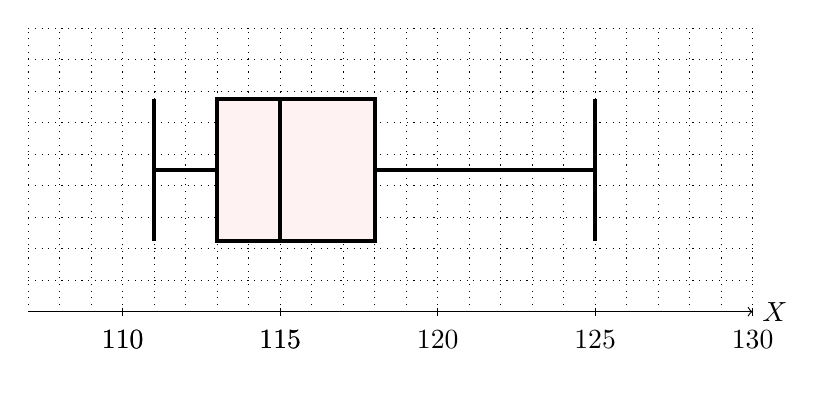
\begin{tikzpicture}[x=0.4cm,y=0.9cm]
         \draw[step=0.4cm,,dotted,color=black] (107,0) grid (130,4);
		\draw[->] (107,0) -- (130,0) node[right] {$X$} ;
		\foreach \X in {110,115,110,115,120,125,130} {
			\draw (\X,0.05cm) -- (\X,-0.05cm) node[below] {$\X\strut$};}
		\draw[ultra thick][fill=red!5] (113,1) rectangle (118,3);
  	\draw[ultra thick] (115,1) -- (115,3);

		\draw[ultra thick] (111,1) -- (111,3);
		\draw[ultra thick] (111,2) -- (113,2);
		\draw[ultra thick] (118,2) -- (125,2);
		%\draw[ultra thick] (4,1) -- (4,3);
		\draw[ultra thick] (125,1) -- (125,3);
			\end{tikzpicture}\\
	\end{center}
 \begin{solution}
     Il manque la médiane à (114 + 114) /2 = 114
 \end{solution}
\vspace{13cm}

\pagesuivante{\ref{micro}}
\newpage . \newpage
\suite{\ref{micro}}

\part[6] Nous apprenons que la plus grande observation (128) est erronée. Nous ne connaissons pas sa valeur, mais nous savons que celle-ci est plus grande que 150. Nous notons cette valeur XXX et nous savons que XXX~$>$~150. Le nouveau jeu de données est donc:

\begin{center}
\begin{tabular}{  c c c c c c c c }
111  &111  &111  &112  &113  &113  &113 \\
113 &115  &115  &115  &115 &115 & 116 \\
116 & 118 & 118 & 119 & 125 &127 & XXX\\
\end{tabular}
\end{center}

À partir de ce nouveau jeu de données, répondez aux questions suivantes. Nous nommons «jeu de données original» celui qui contient l'observation 128 et «nouveau jeu de données» celui qui contient l'observation XXX.

Déterminez si les énoncés suivants sont vrais ou faux. 

\textbf{\textit{Une bonne réponse vaut 2 points, une mauvaise réponse vaut -1 point et une réponse vide vaut 0 point, pour un total minimum de 0 point.}}

\begin{subparts}
\subpart La médiane échantillonnale du nouveau jeu de données est supérieure à celle du jeu de données original.

    \begin{oneparcheckboxes}
        \choice Vrai
        \correctchoice Faux
    \end{oneparcheckboxes}
    
\begin{solution}
    Faux
\end{solution}

\subpart La moyenne échantillonnale du nouveau jeu de données est supérieure à celle du jeu de données original.

    \begin{oneparcheckboxes}
        \correctchoice Vrai
        \choice Faux
    \end{oneparcheckboxes}
    
\begin{solution}
    Vrai
\end{solution}

\subpart La variance échantillonnale du nouveau jeu de données est supérieure à celle du jeu de données original.

    \begin{oneparcheckboxes}
        \correctchoice Vrai
        \choice Faux
    \end{oneparcheckboxes}
    
\begin{solution}
    Vrai
\end{solution}

\end{subparts}
\end{parts}

\newpage . \newpage
\question\label{estimateursPonctuels} 

Soit $X_1, \hdots, X_9$ un échantillon aléatoire d'une variable $X\sim\mathcal{N}(12, 4)$. Nous avons que $X_1, \dots, X_9$ sont indépendantes. 

\begin{parts}
    \part[4] Calculez la probablité que la moyenne échantillonnale soit supérieure à la vraie moyenne $\mu = 12$ par plus de 0,62 écarts-types échantillonnaux. 
    
    \begin{solution}
        \begin{align*}
            P(\overline{X} > \mu + 0,62S)
            &= P(\overline{X} - \mu  > 0,62S) \cr
             &= P\left(\frac{\overline{X} - \mu}{S/\sqrt{n}}  >  \frac{0,62 S}{S/\sqrt{n}}\right) \cr
             &= P\left( T_{n-1} >  0,62 {\sqrt{9}}\right) \cr
             &= P\left( T_{8} > 1,86\right) \cr
             &= 0,05
        \end{align*}
    \end{solution}
\vspace{10cm}
    \part[4] Calculez la probabilité que la variance échantillonnale soit inférieure à 1,09.

    
        \begin{solution}
        \begin{align*}
            P(S^2 > 1,09)
             &= P\left(\frac{(n-1)S^2}{\sigma^2}  > \frac{(n-1)1,09}{\sigma^2}\right) \cr
             &= P\left( \chi_{n-1}^2  > \frac{8\times 1,09}{4}\right) \cr
             &= P\left( \chi_{8}^2  > 2,18 \right) \cr
             &= 0,975
        \end{align*}
    \end{solution}
\end{parts}

\newpage
.

\end{questions}



\end{document} 
